\section{Materials to refactor.}

From abstract:

We describe \complain{invariants} \complain{manifested}
by the 1d family of \complain{Poncelet}
N-gons interscribed between two concentric, axis-aligned, homothetic ellipses.
These are affine images of a regular polygon whereby the circumcircle is sent to an ellipse with fixed semi-axes.

Finally, we compare the \complain{conserved} quantities with \complain{analogues} for N-periodic trajectories in the elliptic billiard (confocal pair). 

\bigskip

The two \complain{classic} \complain{invariants} 
of \complain{elliptic billiard N-periodics}
(1d families of \complain{Poncelet}
$N$-gons interscribed between two confocal ellipses)
are perimeter and \complain{Joachimsthal's integral}
\cite{sergei91}.
\complain{Essencialmente o que esta escrito:
o leitor deveria saber conteudo de \cite{sergei91}
antes de ler este artigo, né?}

In \cite{reznik2020-intelligencer,garcia2020-new-properties}
\complain{new} \complain{invariants}
have been described for the $N=3$ confocal family involving sums and products of \complain{trajectory cosines} as well as a certain area ratio.
These were later generalized and proved for all $N$ (the area ratio only works for odd $N$) \cite{akopyan2020-invariants,bialy2020-invariants,caliz2020-area-product}.


Here we describe \complain{invariants} over the ``homothetic'' Poncelet family: N-gons interscribed between two concentric, axis-aligned, and homothetic ellipses. This is shown side-by-side with a confocal N-periodic in  \cref{fig:confocal_homot}. Of course these can be regarded as the affine image of regular polygons interscribed between two concentric circles (see \cref{fig:affine-regular}) and therefore, one \complain{trivial conservation} is area $A$. 

\begin{figure}
    \centering
    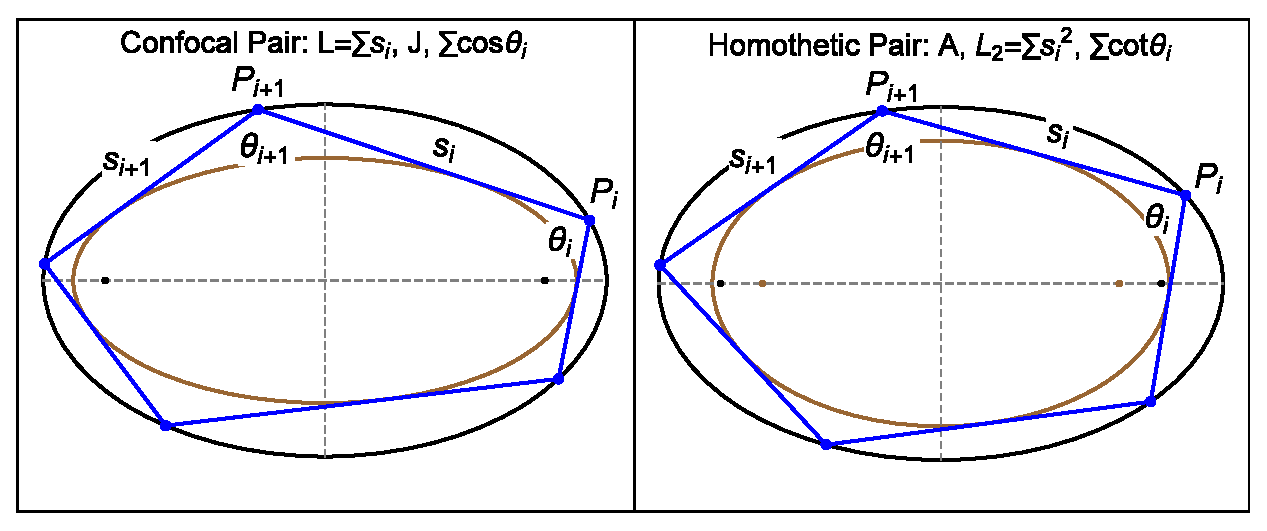
\includegraphics[width=\textwidth]{pics/0010_confocal_homot.eps}
    \caption{\textbf{Left:} A Poncelet pentagon in the confocal pair (elliptic billiard). It classically conserves perimeter $L=\sum{s_i}$ and Joachimsthal's constant $J$ \cite{sergei91}. It also conserves $\sum\cos\theta_i$ \cite{akopyan2020-invariants,bialy2020-invariants,reznik2020-intelligencer}. \textbf{Right:} The family studied herein is identical to a Poncelet one interscribed between two concentric, axis-aligned, non-confocal, homothetic ellipses. It trivially conserves area $A$. We show it also conserves (i) sum of squared sidelengths $s_i^2$ and (ii) sum of {\em cotangents} of the $\theta_i$.}
    \label{fig:confocal_homot}
\end{figure}

\begin{figure}
    \centering
    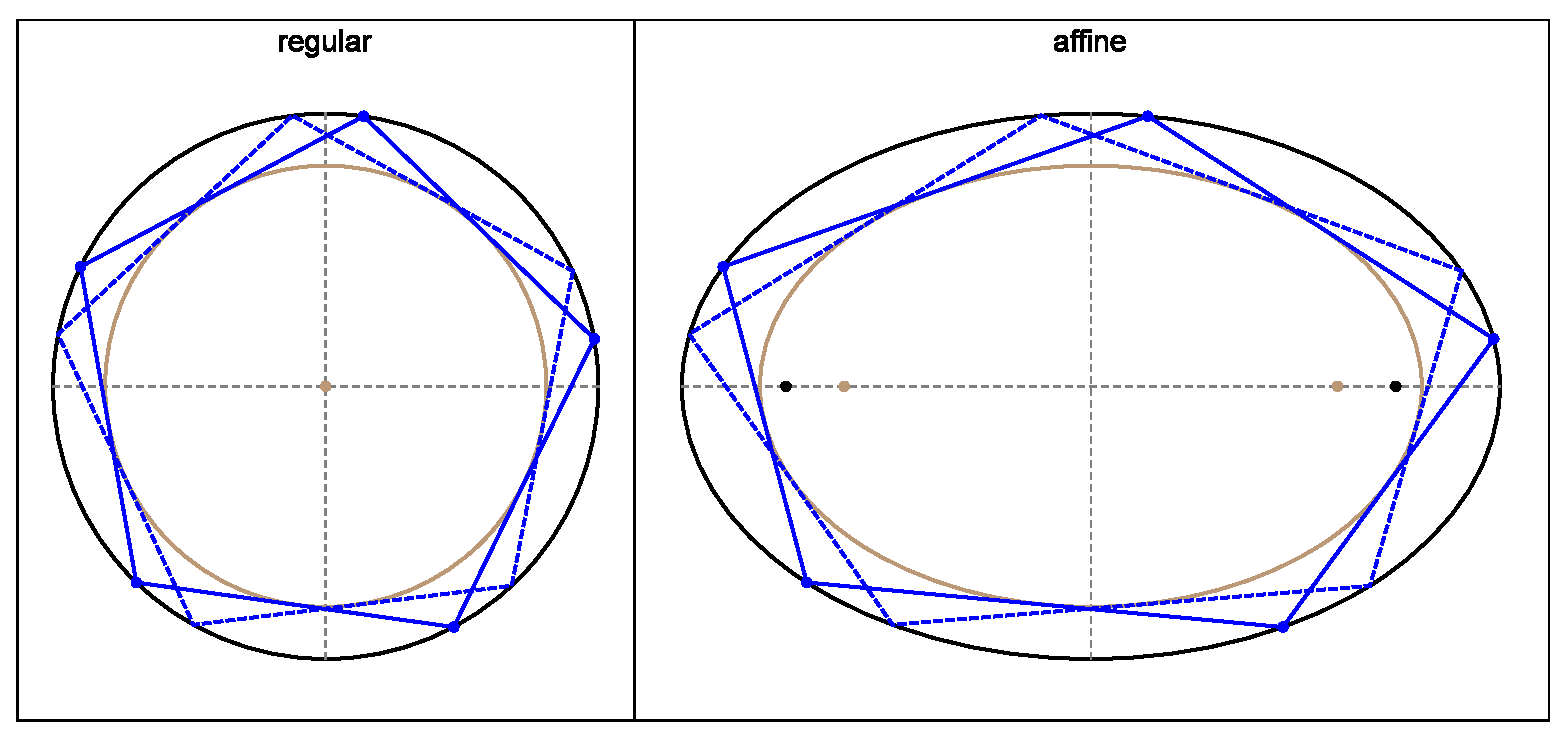
\includegraphics[width=\textwidth]{pics/0030_affine_regular-caustic.eps}
    \caption{The image of a family of regular polygons (left) under a fixed affine transformation are polygons interscribed between two concentric, axis-aligned, homothetic ellipses (right). The latter is sometimes called the Poncelet ``homothetic'' family. In this describe certain Euclidean invariants of the latter.}
    \label{fig:affine-regular}
\end{figure}

Let $P_i,\theta_i,s_i$ denote the vertices, angles, and sidelengths of a homothetic trajectory, $i=1,...,N$. \cref{fig:brocard-n3} illustrates the observation that initiated this work: besides area, $N=3$ homothetics also conserve the sum of {\em squared} sidelengths $s_i^2$ (compare: \complain{confocals} conserve the sum of sidelengths).

Since the \complain{Brocard angle} $\omega$ of a triangle is given by \cite[Brocard Angle, Eqn. 2]{mw}:

\[ \cot\omega=\sum\frac{s_i^2}{4A}=\cot\theta_1+\cot\theta_2+\cot\theta_3 \]
So $N=3$ homothetics are equibrocardial \cite{johnson1960}, i.e., their $\omega$ is constant. Therefore, the sum of cotangents is also invariant  (compare: confocals conserve the sum of cosines).

\begin{figure}
    \centering
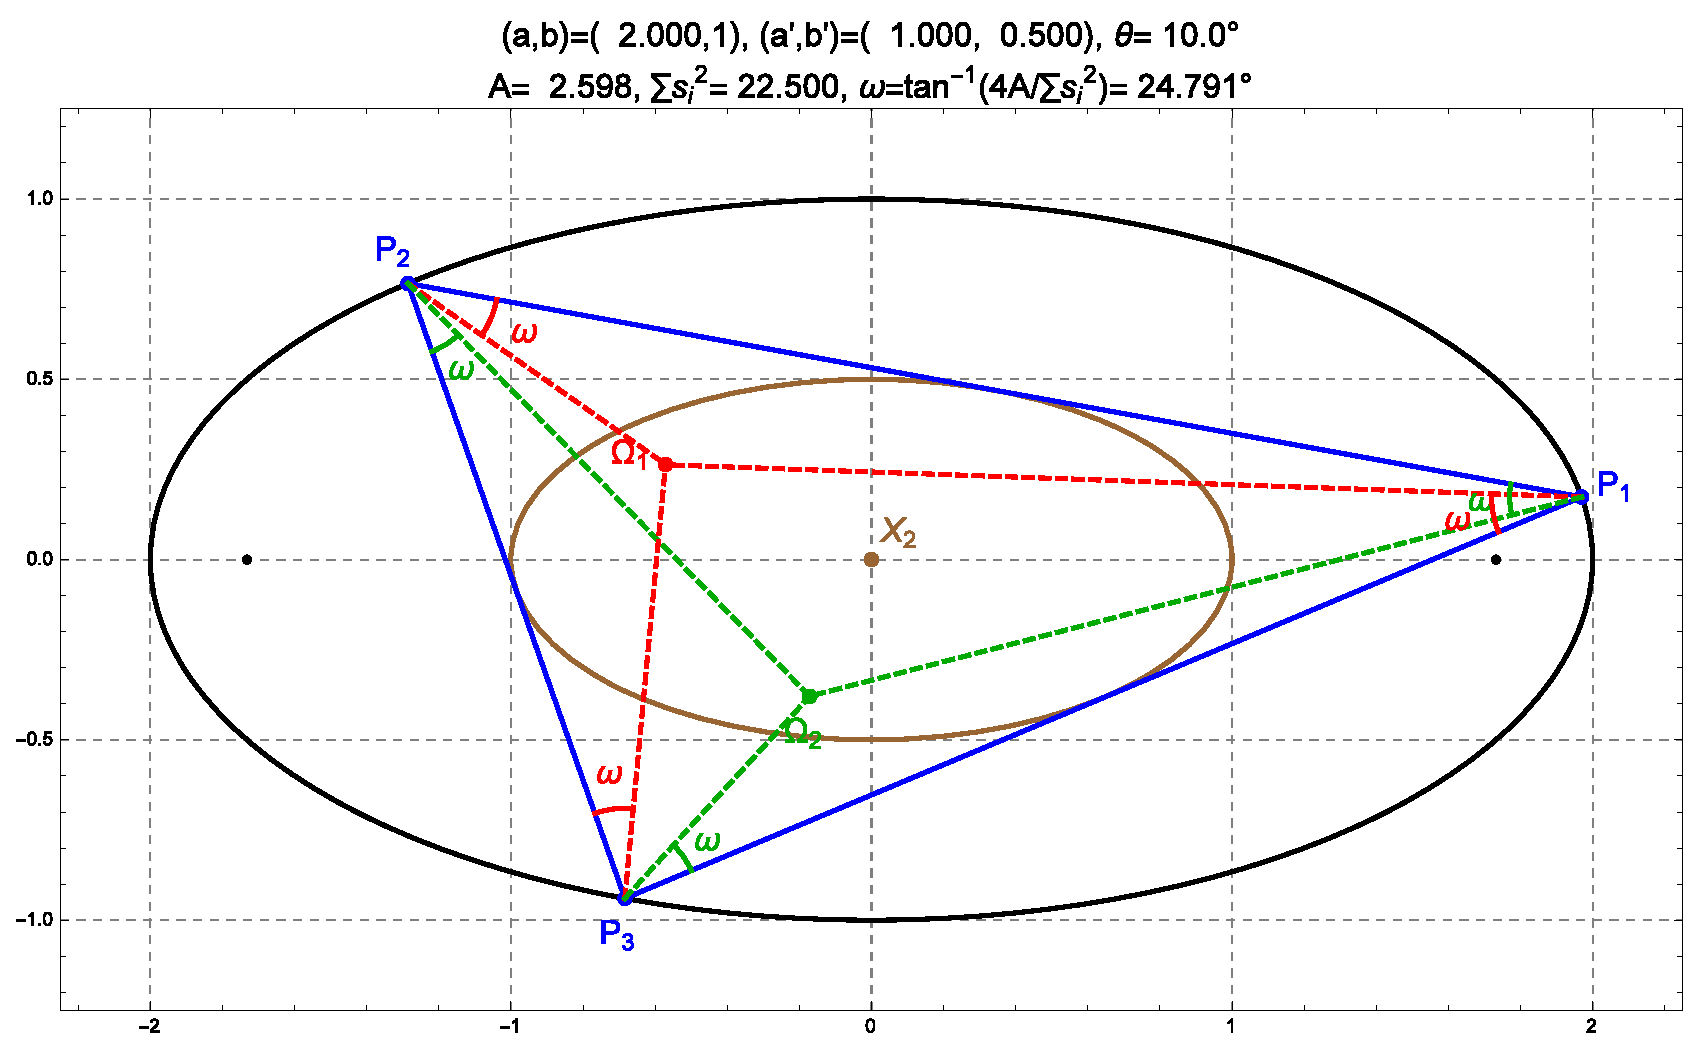
\includegraphics[width=\textwidth]{pics/0040_brocard_n3.eps}
\caption{The family of triangles in the homothetic pair conserve area, sum of squared sidelengths and the Brocard angle $\omega$ which is the particular angle of rotation of sidelengths such that they concur at the two Brocard points $\Omega_1$ and $\Omega_2$. $X_2$ is barycenter which remains stationary over the family at the common center. \href{https://youtu.be/2fvGd8wioZY}{Video 1} and \href{https://youtu.be/13i3JGY-fK4}{Video 2}.}
    \label{fig:brocard-n3}
\end{figure}

Though for \complain{$N>3$ homothetics}
$\omega$ is no longer defined,
we show below that these continue to conserve the sum of sidelengths squared and the sum of cotangents. 

Additionally, we also study invariants of the ``evolute polygon'' whose vertices are fixed linear combinations of the $P_i$ and the centers of curvature. We show invariance of (i) their squared sidelengths (except for $N=4$ or $N=6$), and (ii) their signed area (except for $N=4$).

\textcolor{red}{sergey please check/improve}

